\documentclass[tikz,border=7pt]{standalone}
\usepackage[T1]{fontenc}
\usepackage{lmodern}
\usepackage{helvet}
\renewcommand{\familydefault}{\sfdefault}
\usepackage{amsmath}
\usepackage{xcolor}
\usepackage{tikz}
\usetikzlibrary{
  arrows.meta,
  positioning,
  calc,
  fit,
  shapes.geometric,
  shapes.symbols,
  backgrounds,
  decorations.pathreplacing,
  decorations.pathmorphing,
}

\definecolor{slate}{HTML}{334155}
\definecolor{teal}{HTML}{0D9488}
\definecolor{amber}{HTML}{D97706}
\definecolor{rose}{HTML}{E11D48}
\definecolor{muted}{HTML}{64748B}
\definecolor{line}{HTML}{94A3B8}
\definecolor{pagebg}{HTML}{F8FAFC}
\definecolor{card}{HTML}{FFFFFF}
\definecolor{lightteal}{HTML}{CCFBF1}
\definecolor{lightamber}{HTML}{FEF3C7}
\definecolor{lightrose}{HTML}{FFE4E6}
\definecolor{lightslate}{HTML}{E2E8F0}
\definecolor{blueink}{HTML}{2563EB}
\definecolor{bluewash}{HTML}{DBEAFE}
\definecolor{greenink}{HTML}{16A34A}
\definecolor{greenwash}{HTML}{DCFCE7}
\definecolor{pinkink}{HTML}{DB2777}
\definecolor{pinkwash}{HTML}{FCE7F3}

\tikzset{
  >=Stealth,
  font=\sffamily\scriptsize,
  every node/.append style={text=slate},
  title/.style={font=\sffamily\bfseries\small, text=slate, anchor=west},
  note/.style={font=\sffamily\tiny, text=muted, align=left},
  label/.style={font=\sffamily\tiny, text=muted},
  chip/.style={
    draw=#1,
    fill=#1!12,
    rounded corners=2pt,
    inner sep=2.5pt,
    font=\sffamily\tiny\bfseries,
    text=slate,
  },
  decision/.style={
    shape=diamond,
    aspect=2.1,
    draw=teal,
    fill=lightteal,
    inner sep=1.5pt,
    align=center,
    font=\sffamily\tiny,
    text=slate,
  },
  pics/person/.style 2 args={
    code={
      \fill[#1] (0,0.92) circle (0.18);
      \fill[#1]
        (-0.26,0.68)
        .. controls (-0.34,0.42) and (-0.30,0.18) .. (-0.22,0.02)
        -- (0.22,0.02)
        .. controls (0.30,0.18) and (0.34,0.42) .. (0.26,0.68)
        -- cycle;
      \node[font=\sffamily\tiny\bfseries, text=#1, anchor=north] at (0,-0.08) {#2};
    }
  },
  pics/disk/.style={
    code={
      \fill[lightslate] (0,-0.04) ellipse (0.28 and 0.10);
      \fill[slate] (-0.28,-0.04) rectangle (0.28,0.12);
      \fill[slate] (0,0.12) ellipse (0.28 and 0.10);
      \fill[card] (0,0.14) ellipse (0.11 and 0.04);
    }
  },
}

\begin{document}
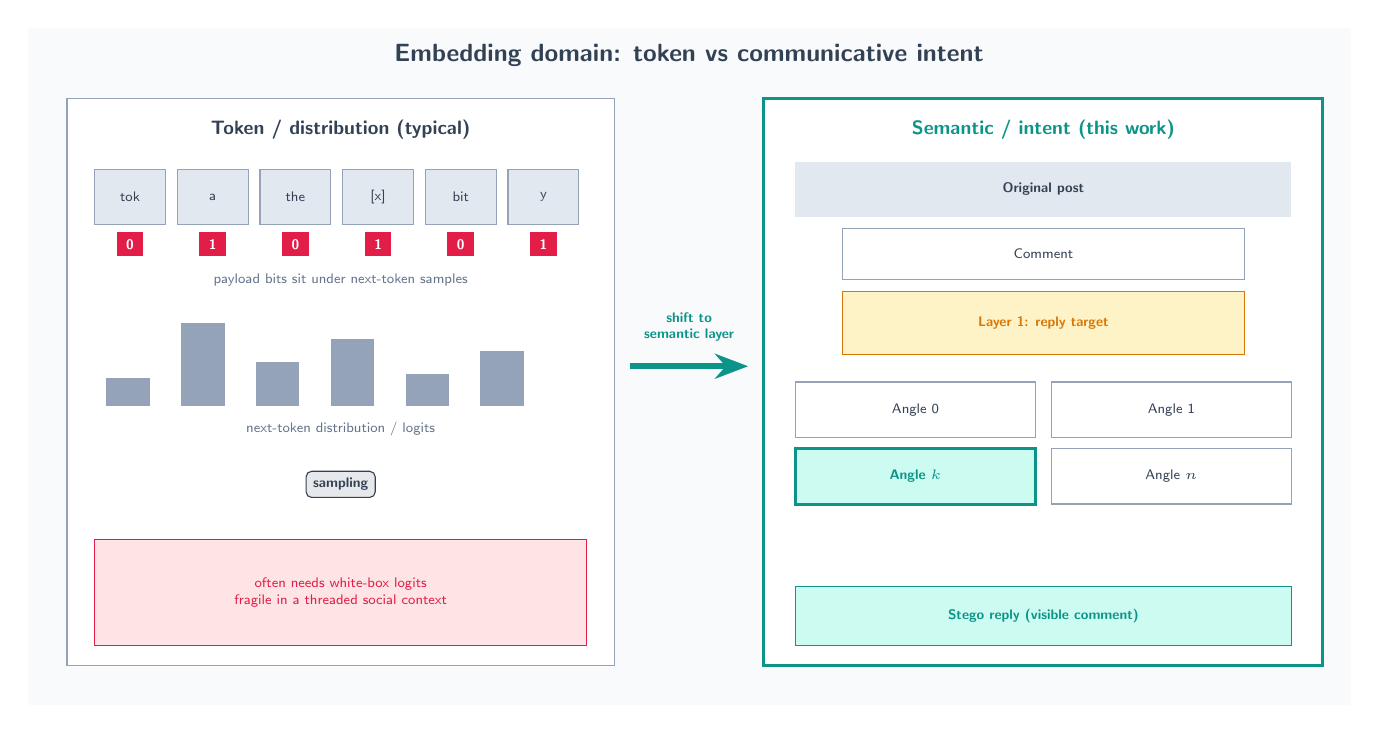
\begin{tikzpicture}[x=1cm,y=1cm]
  \fill[pagebg] (-0.3,-0.25) rectangle (16.5,8.35);
  \node[title, anchor=center] at (8.1,8.00) {Embedding domain: token vs communicative intent};

  % LEFT panel
  \fill[card] (0.2,0.25) rectangle (7.15,7.45);
  \draw[line] (0.2,0.25) rectangle (7.15,7.45);
  \node[font=\sffamily\bfseries\scriptsize] at (3.675,7.05) {Token / distribution (typical)};

  \foreach \i/\tok/\bit in {0/tok/0, 1/a/1, 2/the/0, 3/[x]/1, 4/bit/0, 5/y/1} {
    \pgfmathsetmacro{\xx}{0.55+\i*1.05}
    \fill[lightslate] (\xx,5.85) rectangle (\xx+0.90,6.55);
    \draw[line] (\xx,5.85) rectangle (\xx+0.90,6.55);
    \node[font=\sffamily\tiny] at (\xx+0.45,6.20) {\tok};
    \fill[rose] (\xx+0.28,5.45) rectangle (\xx+0.62,5.75);
    \node[font=\sffamily\tiny\bfseries, text=card] at (\xx+0.45,5.60) {\bit};
  }
  \node[label] at (3.675,5.15) {payload bits sit under next-token samples};

  % logit bars
  \foreach \i/\h in {0/0.35, 1/1.05, 2/0.55, 3/0.85, 4/0.40, 5/0.70} {
    \pgfmathsetmacro{\xx}{0.70+\i*0.95}
    \fill[line] (\xx,3.55) rectangle (\xx+0.55,3.55+\h);
  }
  \node[label] at (3.675,3.25) {next-token distribution / logits};

  \node[chip=slate] at (3.675,2.55) {sampling};
  \fill[lightrose] (0.55,0.50) rectangle (6.80,1.85);
  \draw[rose] (0.55,0.50) rectangle (6.80,1.85);
  \node[font=\sffamily\tiny, text=rose, align=center, text width=5.8cm] at (3.675,1.175) {often needs white-box logits\\fragile in a threaded social context};

  % arrow
  \draw[teal, line width=2pt, ->] (7.35,4.05) -- (8.85,4.05);
  \node[font=\sffamily\tiny\bfseries, text=teal, align=center] at (8.10,4.55) {shift to\\semantic layer};

  % RIGHT panel
  \fill[card] (9.05,0.25) rectangle (16.15,7.45);
  \draw[teal, line width=1.1pt] (9.05,0.25) rectangle (16.15,7.45);
  \node[font=\sffamily\bfseries\scriptsize, text=teal] at (12.60,7.05) {Semantic / intent (this work)};

  \fill[lightslate] (9.45,5.95) rectangle (15.75,6.65);
  \node[font=\sffamily\tiny\bfseries] at (12.60,6.30) {Original post};

  \fill[card] (10.05,5.15) rectangle (15.15,5.80);
  \draw[line] (10.05,5.15) rectangle (15.15,5.80);
  \node[font=\sffamily\tiny] at (12.60,5.475) {Comment};

  \fill[lightamber] (10.05,4.20) rectangle (15.15,5.00);
  \draw[amber] (10.05,4.20) rectangle (15.15,5.00);
  \node[font=\sffamily\tiny\bfseries, text=amber] at (12.60,4.60) {Layer 1: reply target};

  \foreach \lab/\sel/\xx/\yy in {Angle 0/0/9.45/3.15, Angle 1/0/12.70/3.15, Angle $k$/1/9.45/2.30, Angle $n$/0/12.70/2.30} {
    \ifnum\sel=1
      \fill[lightteal] (\xx,\yy) rectangle (\xx+3.05,\yy+0.70);
      \draw[teal, line width=1.1pt] (\xx,\yy) rectangle (\xx+3.05,\yy+0.70);
      \node[font=\sffamily\tiny\bfseries, text=teal] at (\xx+1.525,\yy+0.35) {\lab};
    \else
      \fill[card] (\xx,\yy) rectangle (\xx+3.05,\yy+0.70);
      \draw[line] (\xx,\yy) rectangle (\xx+3.05,\yy+0.70);
      \node[font=\sffamily\tiny] at (\xx+1.525,\yy+0.35) {\lab};
    \fi
  }

  \fill[lightteal] (9.45,0.50) rectangle (15.75,1.25);
  \draw[teal] (9.45,0.50) rectangle (15.75,1.25);
  \node[font=\sffamily\tiny\bfseries, text=teal] at (12.60,0.875) {Stego reply (visible comment)};
\end{tikzpicture}
\end{document}
